\section{Haystack open-source framework}
\label{sec:haystack}
Το \emph{Haystack}\footnote{\url{https://haystack.deepset.ai/overview/intro}} αποτελεί ένα \emph{open-source framework} για την κατασκευή συστημάτων αναζήτησης σε μεγάλο αριθμό εγγράφων. Οι πρόσφατες εξελίξεις στον τομέα της επεξεργασίας φυσικής γλώσσας έδωσαν την δυνατότητα για ανάπτυξη συστημάτων ερωτοαπαντήσεων, ανάκτηση και περίληψη κειμένου και το \emph{Haystack} αποτελεί τη γέφυρα μεταξύ της έρευνας και της υλοποίησης σε πραγματικά συστήματα.

Μερικά από τα κύρια πλεονεκτήματα του είναι η χρήση \emph{NLP} για αναζήτηση χρησιμοποιώντας μοντέλα τελευταίας τεχνολογίας (\emph{state of the art}) από δημοφιλής βιβλιοθήκες όπως το \emph{huggingface}\footnote{\url{https://huggingface.co/}}. Επιπλέον, υποστηρίζει πληθώρα βάσεων δεδομένων ανάμεσα στις οποίες είναι οι \emph{Elasticsearch, Milvus\footnote{\url{https://milvus.io/}}, FAISS\footnote{\url{https://ai.facebook.com/tools/faiss/}}, SQL\footnote{\url{https://www.mysql.com/}}} και άλλες. Τέλος, παρέχει εργαλεία για τη δημιουργία παραδειγμάτων, συλλογή σχολίων χρηστών, αξιολόγηση και \emph{finetuning} μοντέλων. 

Στο \autoref{fig:haystack_concepts} παρουσιάζεται η συνολική δομή ενός συστήματος του \emph{Haystack}. Τα έγγραφα πρώτα δέχονται προ-επεξεργασία, για την πιο αποδοτική αναζήτηση στη βάση δεδομένων, και έπειτα αποθηκεύονται σε αυτή. Από τα πιο σημαντικά κομμάτια του \emph{Haystack} είναι ο \emph{Retriever} και ο \emph{Reader}. Ο \emph{Retriever}, είναι κόμβος ο οποίος λειτουργεί σαν ένα φίλτρο το οποίο ανατρέχει όλα τα έγγραφα που είναι αποθηκευμένα στη βάση δεδομένων και αναζητά εκείνα τα έγγραφα που μοιάζουν πιο πολύ με την εισερχόμενη ερώτηση. Συνήθως χρησιμοποιείται σε συνδυασμό με τον \emph{Reader} ο οποίος είναι υπεύθυνος να ανατρέξει τα υποψήφια έγγραφα που επέστρεψε ο \emph{Retriever} και να επιστρέψει τις απαντήσεις στις εισόδους του συστήματος. Πρακτικά, εδώ ενσωματώνεται το NLP μοντέλο που θα χρησιμοποιηθεί για να αναζητήσει την απάντηση στα έγγραφα που επιστράφηκαν από τον \emph{Retriever}.

\begin{figure}[!ht]
  \centering
  \captionsetup{justification=centering}
  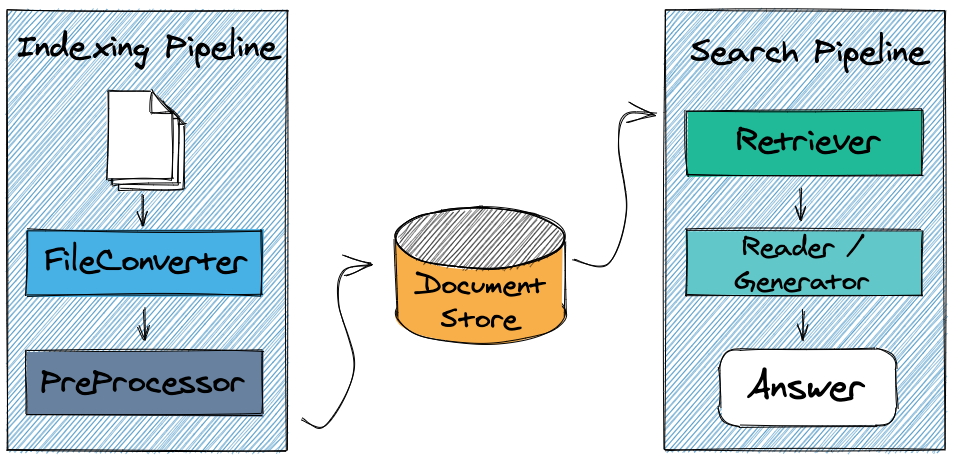
\includegraphics[width=0.7\textwidth]{images/chapter3/concepts_haystack_handdrawn.png}
  \captionsource{Βασική δομή \emph{Haystack}}{\url{https://haystack.deepset.ai/overview/intro}}
  \label{fig:haystack_concepts}
\end{figure}
\noindent